% === [ Design ] ===============================================================

% <howto>
% * Justify, evaluate, recognize limitations of.
%
% * Analytical writing
%    - Why did you do X that way?
%    - Why did you do Y but not Z?
%    - What was important and what not?

% <howto>
% * If you were to implement the system in another language, which aspects of
%   the design would remain?
% * Which are the guiding design principles?
% * Describe the general system architecture; which components interact, how,
%   and why?
% * How are the individual components designed? (once again, which aspects
%   remain if you implemented them in another language?)

\begin{quote}
	\textit{``The whole is more than the sum of its parts.''} --- Anonymous
\end{quote}

\section{Design}
\label{sec:design}

The principle of separation of concern has had a core influence on the design of the decompilation system. It has motivated a system architecture based on the composition of independent and self-contained components. End-users may either use the individual component in separation, or combine a set of components into a custom decompilation pipeline.

Several smaller components may conceptually be arranged in a pipeline of stages which transform, massage or interpret the input in a certain way to solve larger tasks. A well composed pipeline is capable of solving more complex problems than each of its components, problems which may not even have been envisioned by the original component authors~\cite{simplicity_and_collaboration}. This idea is embodied in the Unix philosophy and it has influenced software construction profoundly~\cite{art_of_unix}. Furthermore, systems which expose their individual components to end-users facilitate dynamic workflows, as they enable users to adapt and extend each part of the system by adding, removing, replacing or refining components in one or more stages of the pipeline.

To enforce a strict separation of concerns, each component is given access to the least amount of information required to successfully accomplish its task (e.g. the control flow analysis stage operates on CFGs and is unaware of the underlying code).

The design of the decompilation system must allow language-agnostic interaction between components written in different programming languages (refer to the aim of the project in section~\ref{sec:intro_project_aim_and_objectives}). This requirement has been satisfied by communicating through well-defined input and output (e.g. JSON, DOT, LLVM IR). A more detailed view of the system architecture is presented in section~\ref{sec:design_system_architecture}.

% === [ Subsections ] ==========================================================

% --- [ System Architecture ] --------------------------------------------------

% <howto>
% * the overall structure of the software system (architecture)

% <howto>
% * Software architecture is concerned with deciding what has to be done, and which program component is going to do it (how something is done is left to the detailed design phase, below)
% * It effectively defines the interface between the programs of the system.
% * This stage does not need to consider non-functional requirements (e.g. response time, reliability, maintainability).

\subsection{System Architecture}
\label{sec:design_system_architecture}

The decompilation pipeline conceptually consists of three modules which separate the general decompilation tasks (e.g. control flow analysis) from concerns related to the source language and the target language. Firstly, the front-end translates a variety of source languages (e.g. x86 or ARM assembly, C or Haskell source code, …) to LLVM IR by utilizing several independent open source projects. Secondly, the middle-end structures the LLVM IR by identifying high-level control flow primitives in the CFGs generated from the intermediate representation. Lastly, the back-end translates the structured LLVM IR into a high-level target programming language (e.g. Go). The interaction between these modules is visualised in figure \ref{fig:decompilation_pipeline}, and the individual components of the front-end, middle-end and back-end modules are further described in section \ref{sec:design_front-end_components}, \ref{sec:design_middle-end_components} and \ref{sec:design_back-end_components} respectively.

\begin{figure}[htbp]
	\begin{center}
		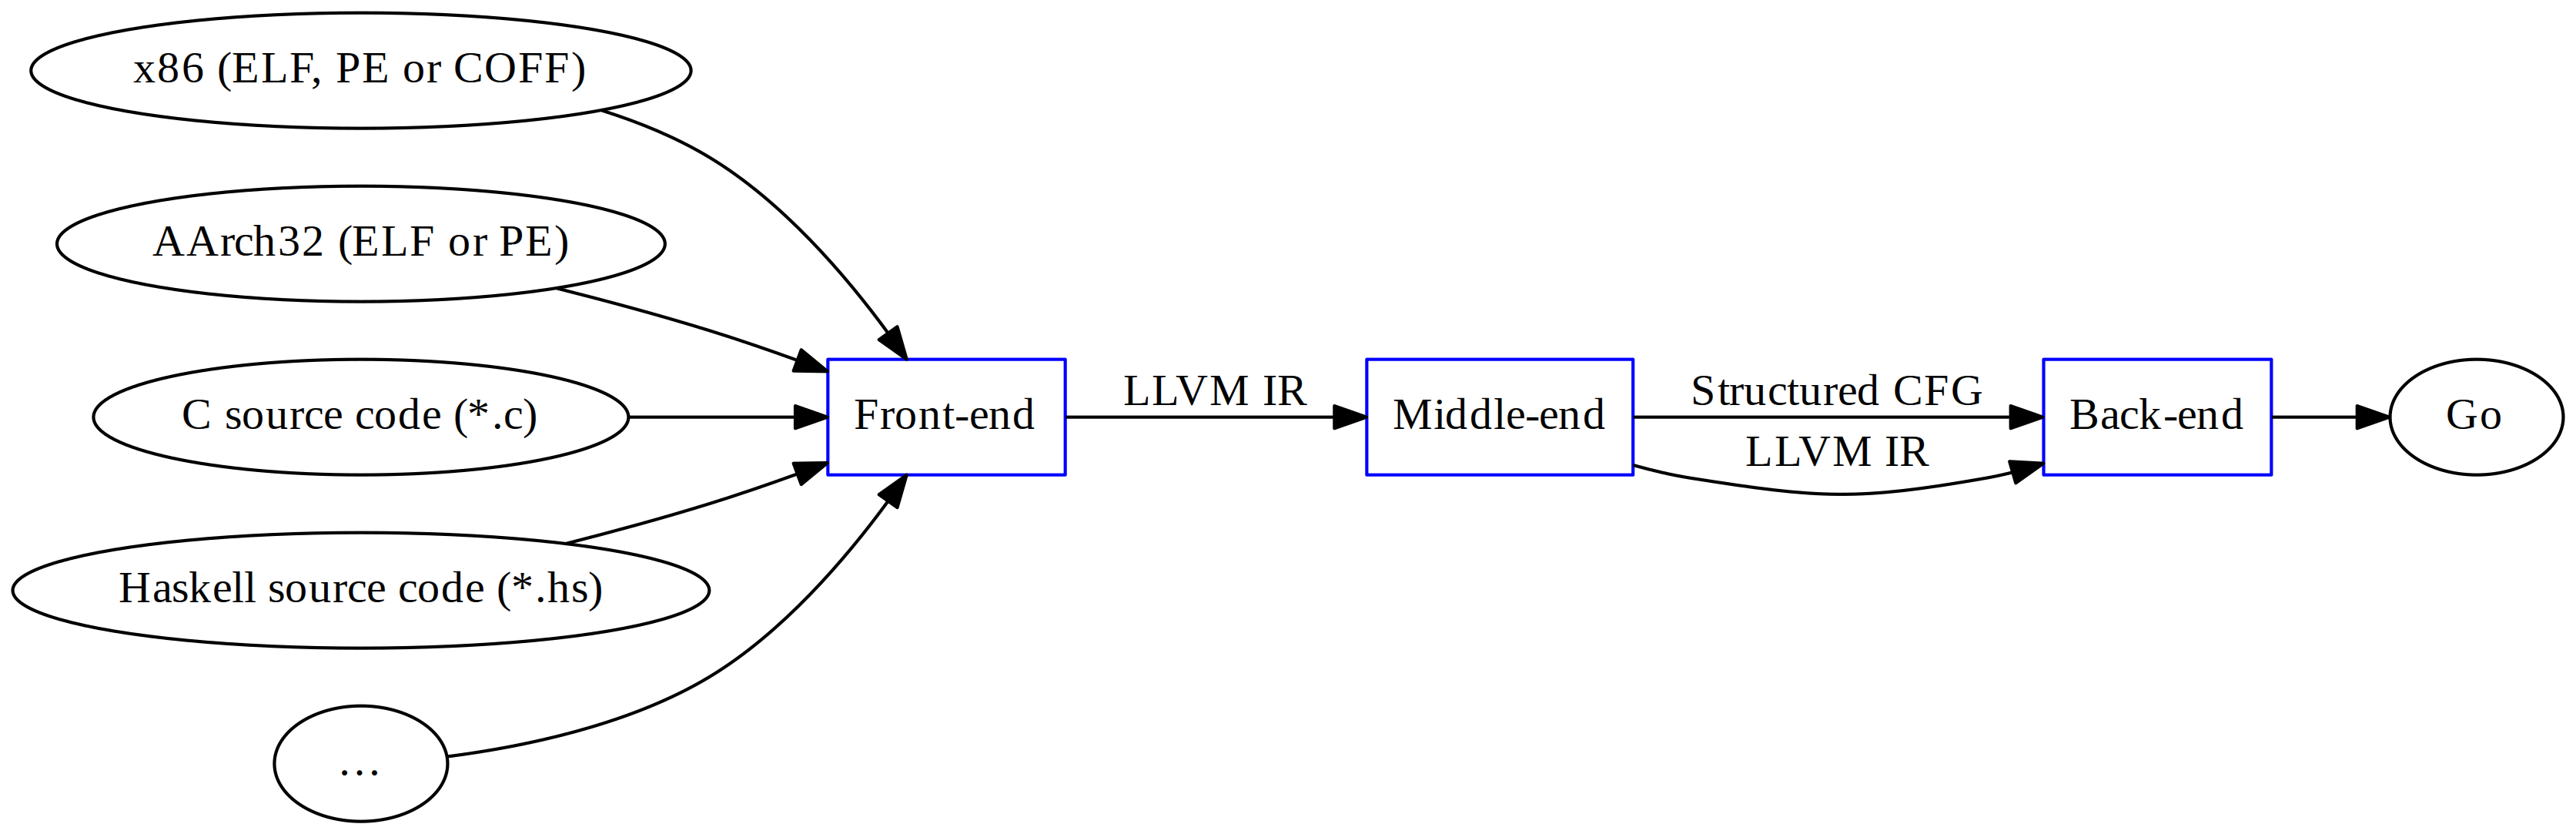
\includegraphics[width=\textwidth]{inc/6_design/decompilation_pipeline.png}
		\caption{The front-end of the decompilation pipeline translates a variety of inputs (e.g. native code or source code) to LLVM IR; the middle-end structures the LLVM IR through control flow analysis; and the back-end translates the structured LLVM IR to a high-level programming language (e.g. Go).}
		\label{fig:decompilation_pipeline}
	\end{center}
\end{figure}

The main benefit with this decompiler architecture is that it scales well when implementing support for additional source languages (e.g. MIPS or PowerPC assembly) and target languages (e.g. Python), as the general decompilation tasks only have to be implemented once. The decompiler architecture is an adaptation of the one presented by C. Cifuentes back in 1994 (as described in section \ref{sec:lit_review_decompilation_phases}), which was heavily inspired by the architecture of compilers that separated general optimisation tasks (e.g. constant propagation) from concerns related to the source programming language (e.g. C) and the target computer architecture (e.g. x86). The compiler architecture has been proven so effective at separating concerns that it remains in use today by several production-quality compilers \cite{llvm_architecture,gcc_architecture}.

% --- [ Front-end Components ] -------------------------------------------------

\subsection{Front-end Components}
\label{sec:front-end_components}

% TODO: Rewrite and clarify.

The front-end module is responsible for converting the input into LLVM IR. Two common scenarios exists, converting binary files (e.g. executables, shared libraries and relocatable object code) and converting source code (e.g. C, Haskell, Rust, …) into LLVM IR. The first scenario is presented in section \ref{sec:design_native_code_to_llvm_ir} and the second in section \ref{sec:compilers}.

% --- [ Subsubsections ] -------------------------------------------------------

% ~~~ [ Native Code to LLVM IR ] ~~~~~~~~~~~~~~~~~~~~~~~~~~~~~~~~~~~~~~~~~~~~~~~

\subsubsection{Native Code to LLVM IR}
\label{sec:design_native_code_to_llvm_ir}

There exist several open source projects which translate native code (e.g. x86 assembly of shared libraries in the PE file format) into LLVM IR. Three such projects have been reviewed in section \ref{sec:rel_work_native_code_to_llvm_ir}, which support different input file formats and machine architectures. These projects may be used as-is by the front-end module to translate low-level source languages into LLVM IR, as illustrated in figure \ref{fig:front-end_binary}.

\begin{figure}[htbp]
	\begin{center}
		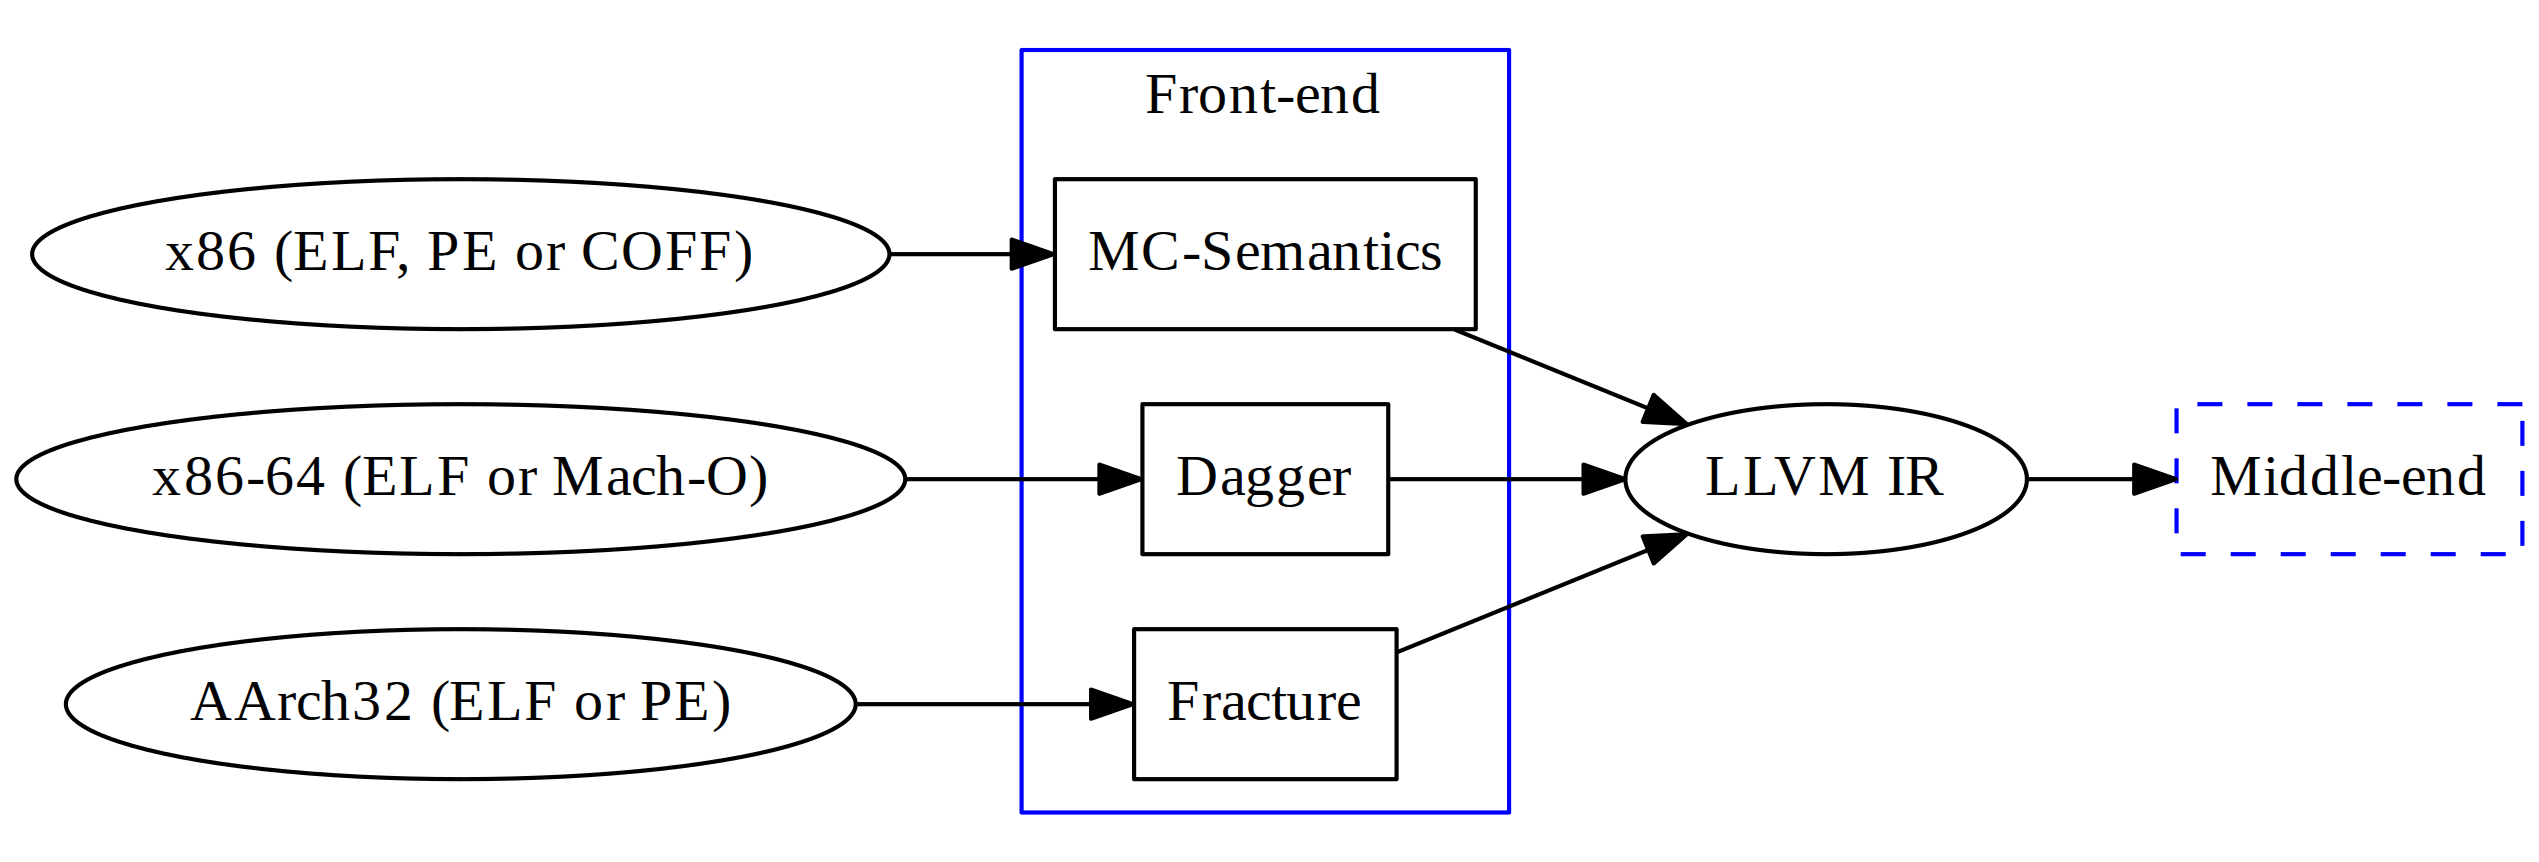
\includegraphics[width=\textwidth]{inc/6_design/front-end_binary.png}
		\caption{The three open source projects MC-Semantics, Dagger and Fracture translate native code of various architectures (e.g. x86, x86-64 and ARM) and file formats (e.g. ELF, PE, COFF and Mach-o) to LLVM IR.}
		\label{fig:front-end_binary}
	\end{center}
\end{figure}

% ~~~ [ Compilers ] ~~~~~~~~~~~~~~~~~~~~~~~~~~~~~~~~~~~~~~~~~~~~~~~~~~~~~~~~~~~~

\subsubsection{Compilers}
\label{sec:design_compilers}

One important aspect of utilizing the IR of a compiler framework, is that the decompilation pipeline automatically gains support for transpilation (i.e. translating one programming language into another) in addition to reverse compilation. An increasing number of open source compilers (e.g. Clang, GHC, \texttt{rustc}) are capable of translating a range of source languages (e.g. C, Haskell, Rust) into LLVM IR. These compilers may be used as-is by the front-end module (see figure \ref{fig:front-end_source}), thereby extending the supported source languages of the decompilation pipeline. Using this approach, the decompilation pipeline may translate $ n $ source languages into $ m $ target languages by implementing $ n + m $ front-end and back-end modules, instead of $ n \cdot m $ transpilers.

\begin{figure}[htbp]
	\begin{center}
		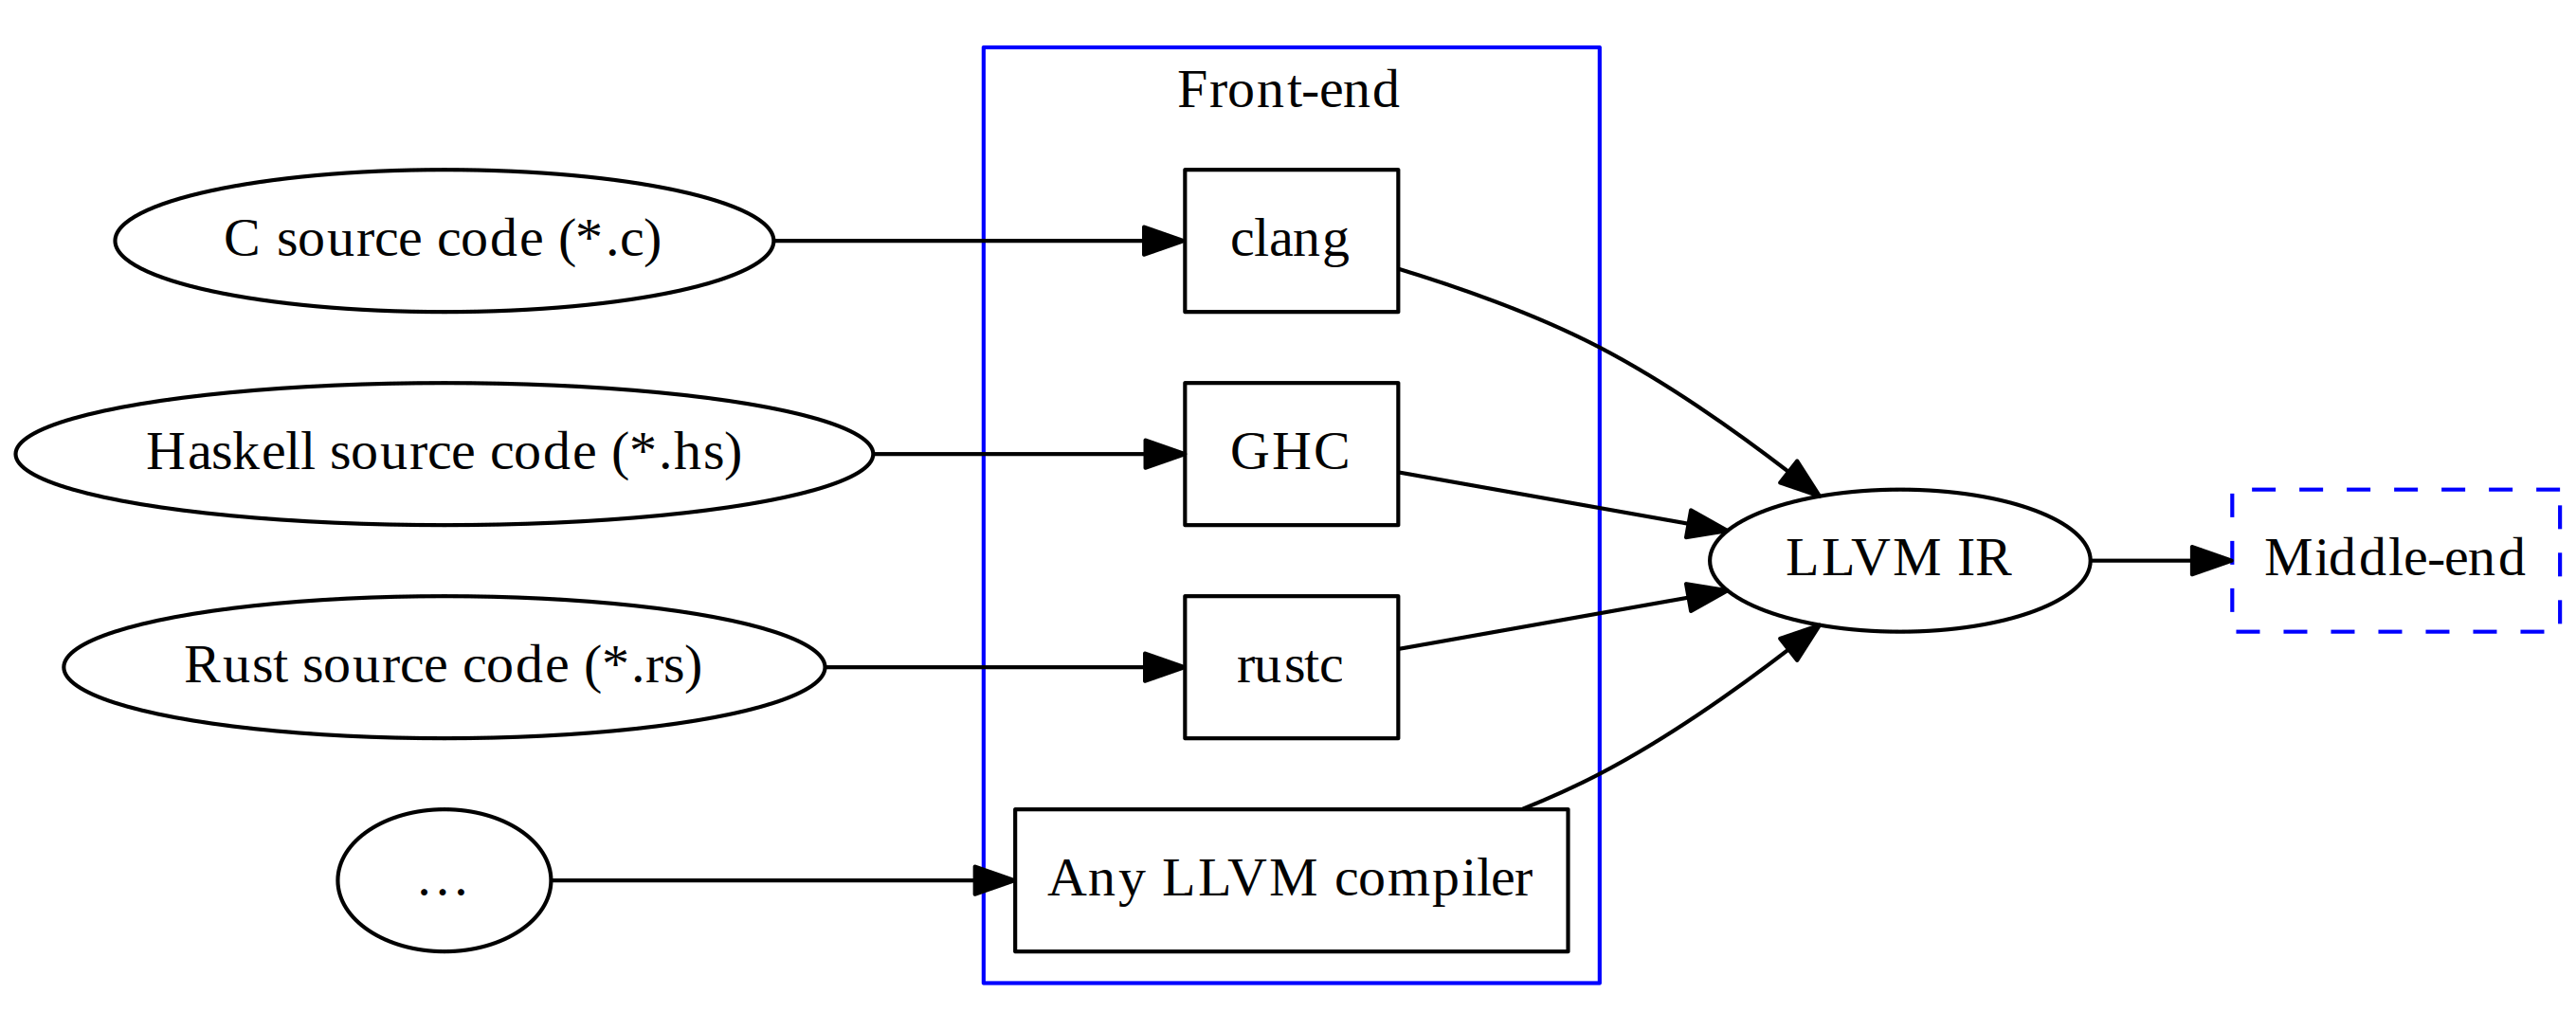
\includegraphics[width=\textwidth]{inc/6_design/front-end_source.png}
		\caption{Several open source compilers translate high-level programming languages into LLVM IR. Three such compilers are Clang, the Glasgow Haskell Compiler and the Rust compiler which translate C, Haskell and Rust respectively into LLVM IR.}
		\label{fig:front-end_source}
	\end{center}
\end{figure}

Another important aspect of utilizing LLVM IR, is that a wide range of optimizations have been implemented already by the LLVM compiler framework. This allows the front-end components to focus on translating the source languages into LLVM IR, without having to worry about producing highly optimised output. The LLVM IR may later be optimised by invoking the \texttt{opt} tool of LLVM to remove dead code, propagate constants, and promote memory accesses to registers, for instance.


% --- [ Middle-end Components ] ------------------------------------------------

% <howto>
% * more detailed design of individual components (design)

% <howto>
% * The intention is that the design should be detailed enough to provide a good guide for actual coding, including details of any particular algorithms to be used.

\subsection{Middle-end Components}

% TODO: Visualize the dependency graph of the "restructure" tool and describe in detail what input it expects and what output it produces.

% TODO: Write about. Input and output LLVM IR to operate well with components written in other languages. Output LLVM IR with information about high-level control structures stored in the basic block names or in metadata.

% TODO: Mention package division.

% TODO: Rewrite and clarify.

The middle-end is responsible for lifting the LLVM IR to a high-level representation through a series of decompilation passes. The \texttt{ll2dot} tool generates a CFG (in the DOT file format) for each function of a given LLVM IR input file. The \texttt{restructure} tool searches for subgraph isomorphisms of control flow primitives in a given CFG. Once located the nodes identified subgraph are merged into a single node which is labeled with the high-level control flow primitive. Successive iterations continue to simplify the CFG until only one node is left, at which point the high-level control flow primitive has been recovered. Should the \texttt{restructure} tool fail to reduce the graph into a single node, the graph is considered irreducible with regards to the supported high-level control flow primitives. The interaction between the front-end, the \texttt{ll2dot} and \texttt{restructure} tools of the middle-end and the back-end is illustrated in figure \ref{fig:middle-end}.

% TODO: Write about the choice of subgraph isomorphism search algorithm. The
% properties of the control flow graph allows us to optimize.
%
% \cite{subgraph_isomorphism_algorithms}

\begin{figure}[htbp]
	\begin{center}
		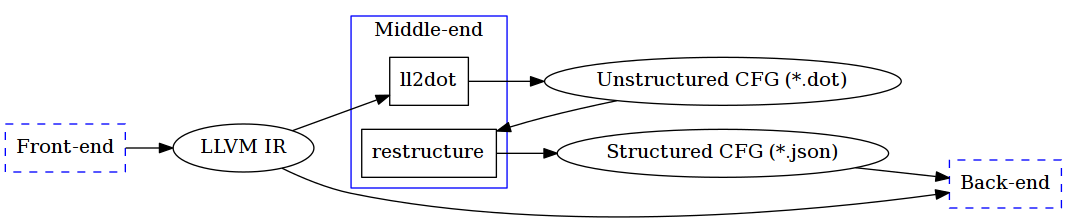
\includegraphics[width=\textwidth]{inc/middle-end.png}
		\caption{foo}
		\label{fig:middle-end}
	\end{center}
\end{figure}

% ~~~ [ Control Flow Graph Generation ] ~~~~~~~~~~~~~~~~~~~~~~~~~~~~~~~~~~~~~~~~

\subsubsection{Control Flow Graph Generation}
\label{sec:design_control_flow_graph_generation}

The control flow graph generation component generates a CFG for each function of a given LLVM IR assembly file. As described in section \ref{sec:lit_review_llvm_ir}, a function definition in LLVM IR consists of a set of basic blocks; and a basic block consists of zero or more non-branching instructions followed by a terminating instruction (such as \texttt{br} or \texttt{ret}) which changes the control flow. Therefore, the control flow graph generation component may focus on analysing the last instruction of each basic block, as they will determine the control flow.

To generate the CFG of a given function, a directed graph is created and populated with one node per basic block, and with zero or more directed edges between the nodes of the graph. The node names are determined by the basic block labels, and the directed edges are determined by the terminating instructions, as illustrated in figure \ref{fig:cfg_gen_example}.

\begin{figure}[htbp]
	\centering
	\begin{subfigure}[ht]{0.54\textwidth}
		\lstinputlisting[language=llvm, style=nasm, tabsize=2]{inc/cfg_gen_example.ll}
	\end{subfigure}
	\enskip
	\begin{subfigure}[ht]{0.22\textwidth}
		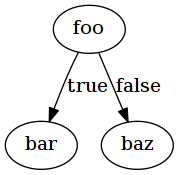
\includegraphics[width=\textwidth]{inc/cfg_gen_example.png}
	\end{subfigure}
	\caption{The return instructions of basic block \texttt{bar} and \texttt{baz} produces no directed edges, while the conditional branch instruction of basic block \texttt{foo} produces two directed edges, one for each target branch (i.e. \texttt{bar} and \texttt{baz}).}
	\label{fig:cfg_gen_example}
\end{figure}


The \texttt{ll2dot} tool generates CFGs from LLVM IR in the DOT file format, which is a well-defined textual representation of graphs used by the Graphviz project. One benefit of expressing CFGs in this format, is that the existing Graphviz tools may be facilitated to produce image representations of the CFGs; as demonstrated in appendix \ref{app:control_flow_graph_generation_example}.

% ~~~ [ Control Flow Analysis ] ~~~~~~~~~~~~~~~~~~~~~~~~~~~~~~~~~~~~~~~~~~~~~~~~

\subsubsection{Control Flow Analysis}
\label{sec:design_control_flow_analysis}

The key idea behind the control flow analysis (see section \ref{sec:control_flow_analysis}), is that high-level control flow primitives may be represented using directed graphs. The problem of structuring low-level code may therefore be rephrased as the problem of identifying subgraphs (e.g. the graph representation of high-level control flow primitives) in graphs (e.g. the CFGs of low-level code) without considering node names, as illustrated in figure \ref{fig:representation_and_identification_of_primitive}. This problem is generally referred to as \textit{subgraph isomorphism search} and has been well studied \cite{subgraph_isomorphism_algorithms}. Rephrasing the problem in this manner aligns with the design principle of giving each component access to the least amount of information required to successfully accomplish its task. The control flow analysis component is only given access to control flow information (e.g. CFGs), and is oblivious of the underlying LLVM IR. This enables the component to be reused as-is when analyzing the control flow of other languages, such as REIL.

\begin{figure}[htbp]
	\centering
	\begin{subfigure}[ht]{0.10\textwidth}
		\lstinputlisting[language=go, style=go, breaklines=false, numbers=none]{poster/inc/if.c}
		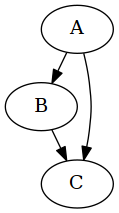
\includegraphics[width=\textwidth]{poster/inc/if.png}
	\end{subfigure}
	\enskip
	\begin{subfigure}[ht]{0.18\textwidth}
		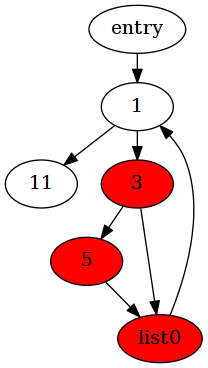
\includegraphics[width=\textwidth]{poster/inc/foo.png}
	\end{subfigure}
	\caption{The left side contains the pseudo-code (top left) and graph representation (bottom left) of an if-statement; if \texttt{A} is true then do \texttt{B} followed by \texttt{C}, otherwise do \texttt{C}. The right side highlights (in red) an identified isomorphism of the if-statement's graph representation, in the CFG of the \texttt{main} function presented in appendix \ref{app:clang_example}.}
	\label{fig:representation_and_identification_of_primitive}
\end{figure}

The \texttt{restructure} tool uses subgraph isomorphism search algorithms to locate isomorphisms of the graph representations of high-level control flow primitives in the CFG of a given function. The CFG is simplified by recursively replacing the identified subgraphs with single nodes until the entire CFG has been reduced into a single node; a step-by-step demonstration of which is presented in appendix \ref{app:control_flow_analysis_example}. By recoding the node names of the identified subgraph isomorphisms and the name of their corresponding high-level control flow primitives, a structured CFG may be produced in which all nodes are known to belong to a high-level control flow primitive; as demonstrated in appendix \ref{app:restructure_example}.

The pseudo-code and graph representations of the supported high-level control flow primitives are presented in figure \ref{fig:graph_representations} of section \ref{sec:control_flow_analysis}. Should the control flow analysis fail to reduce a CFG into a single node, the CFG is considered irreducible with regards to the supported high-level control flow primitives, in which case a structured CFG cannot be produced.

The \texttt{restructure} tool relies entirely on subgraph isomorphism search to produce structured CFGs (in JSON format) from unstructured CFGs (in the DOT file format). The supported high-level control flow primitives are defined using DOT files, thus promoting a data-driven design which separates data regarding the primitives from the implementation of the \texttt{restructure} tool. A major benefit with this approach is that the \texttt{restructure} tool may search for any high-level control flow primitive that can be expressed in the DOT file format, without any modification to the source code.

One limitation with this approach is that it does not support graph representations of high-level control flow primitives with a variable number of nodes, as they cannot be described in the DOT file format. For this reason, the \texttt{restructure} tool does not support the recovery of n-way conditionals (e.g. \texttt{switch}-statements). Furthermore, the current design enforces a single-entry/single-exit invariant on the graph representation of high-level control flow primitives. This prevents the recovery of infinite loops, as their graph representation has no exit node. A discussion of how these issues may be mitigated in the future is provided in section \ref{sec:design_validation}.


% --- [ Back-end Components ] --------------------------------------------------

\subsection{Back-end Components}
\label{sec:design_back-end_components}

The back-end module translates structured LLVM IR into a target high-level programming language, using two distinct stages. Firstly, the code generation stage translates LLVM IR into unpolished Go code by converting the individual instructions into equivalent Go statements and creating high-level control flow primitives for the various basic blocks, using the information of the structured CFGs (see section~\ref{sec:design_control_flow_analysis}). Secondly, the post-processing stage improves the quality of the unpolished Go code, through a series of source code transformations. The interaction between the middle-end, and the \texttt{ll2go} and \texttt{go-post} tools of the back-end is illustrated in figure~\ref{fig:back-end}.

\begin{figure}[htbp]
	\begin{center}
		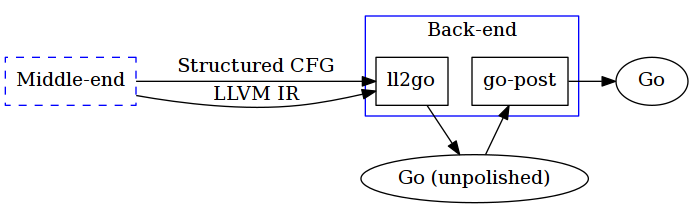
\includegraphics[width=0.8\textwidth]{inc/6_design/back-end.png}
		\caption{The back-end module decompiles structured LLVM IR into Go source code, using two components. The \texttt{ll2go} tool translates structured LLVM IR assembly into unpolished Go code, which is post-processed by the \texttt{go-post} tool to improve the quality of the output.}
		\label{fig:back-end}
	\end{center}
\end{figure}

The clear distinction between the two back-end stages aligns with the design principle of separation of concern. The code generation stage may focus on converting LLVM IR into equivalent Go code, without having to worry about the quality of the produced code. Similarly, the post-processing stage may focus on simplifying the Go code and make it more idiomatic, without any knowledge of the underlying LLVM IR. This enables the post-processing component to be reused as-is by other projects to improve the quality of Go code.

A tighter integration between the two stages could potentially produce a higher quality output, but there are no known issues preventing the decoupled stages from producing output of equivalent quality.

The decompilation pipeline aims to keep the back-end module as simple as possible, by delegating general decompilation tasks (e.g. control flow analysis, data flow analysis) to the middle-end module. This reduces the efforts required to implement additional back-ends, which add support for new target programming languages (e.g. Python).

% --- [ Subsubsections ] -------------------------------------------------------

% ~~~ [ Post-processing ] ~~~~~~~~~~~~~~~~~~~~~~~~~~~~~~~~~~~~~~~~~~~~~~~~~~~~~~

\subsubsection{Post-processing}
\label{sec:design_post-processing}

The post-processing stage post-processes the unpolished Go source code from the earlier stages of the decompilation pipeline, by applying a set of source code transformations. The \texttt{go-post} tool improves the quality of Go source code by declaring unresolved identifiers, applying Go conventions for exit status codes, propagating temporary variables into expressions, simplifying binary operations, removing dead assignment statements, and promoting the initialisation statement and post-statement of for-loops to the loop header; as demonstrated by the step-by-step refinement of the unpolished source code in presented appendix~\ref{app:post-processing_example}.


